% !TEX root = ../thesis_main.tex
\chapter{Introduction}

Carbon allotropes such as graphene, fullerenes, and carbon nanotubes have attracted substantial interest due their unique properties and their exemplary use as model systems for investigations of many-body physics in low-dimensional systems \cite{zaytseva2016carbon, nanot2012optoelectronic, soavi2016ultrafast}. In particular, carbon nanotubes (CNT) have shown great promise for applications in next-generation optoelectronic devices and have established a role as one of many leading candidate materials to replace other conventional semiconducting materials in such applications \cite{nanot2012optoelectronic}. Some of these applications include terahertz polarizers \cite{ren2009carbon}, transistors \cite{qiu2017scaling}, light-emitting devices \cite{liu2015electrically}, and solar cells \cite{kongkanand2007single}. Additionally, CNTs also exemplify features of one-dimensional (1-D) materials.

\begin{figure}[H]
	\centering
	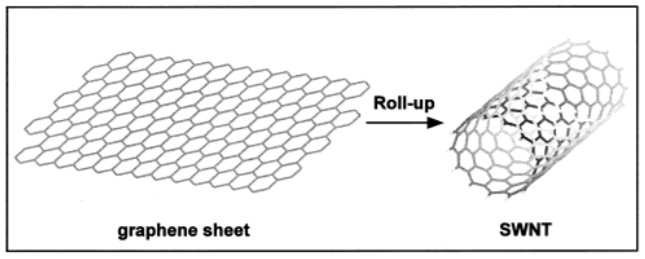
\includegraphics[scale=0.8]{images/chapter_intro/rolled_up_graphene.png}
	\caption{Schematic showing how a 2D sheet of graphene is rolled to form a hollow nanotube. Reproduced and modified from Ref \cite{odom2000structure}.}
\end{figure}

CNTs are best visualized as two-dimensional sheets of graphene that have been rolled up to form hollow, cylindrical structures \cite{odom2000structure,charlier2007electronic}. Their 1-D character arises due to their unusual aspect ratios as CNTs can have diameters of 1 - 3 nanometers whilst possessing lengths of a least one micrometer  \cite{zaytseva2016carbon, ando1997excitons}. This essentially confines their electrons to move only in one direction and significantly enhances electron-electron interactions \cite{ando1997excitons}. Moreover, CNTs can behave as either metals or semiconductors depending on their crystal structure. Owing to such features, CNTs therefore manifest atypical, anisotropic optical and electronic properties \cite{weismanKonoBook}.

Ultrafast spectroscopy provides a means of investigating the microscopic phenomena associated with these features. This technique incorporates the use of ultrashort laser pulses to resolve microscopic dynamics occuring on femtosecond timescales \cite{shah1996ultrafast}. The results reported by similar studies in the past have been partially obfuscated by the quality of samples that were studied. More specifically, these studies used samples containing an ensemble of several different species of carbon nanotubes. As a result, the optical responses of different nanotubes mix together, making it harder to distinguish between the dynamics associated with each species. However, recent developments in sample preparation techniques have made high-purity, single-chirality samples more accessible \cite{ichinose2017extraction}.

\section{Outline}

This thesis focuses on the use of ultrafast spectroscopy to investigate the carrier dynamics of high-purity, CNT samples. Chapter 2 provides a more thorough introduction to the some of the basic properties of carbon nanotubes. Chapter 3 further explores prior ultrafast spectroscopy studies of carbon nanotubes. Chapter 4 illustrates the relevant experimental procedures used in this work. Chapter 5 presents coherent processes that have been observed in CNTs. Finally, Chapter 6 discusses dynamics that occur after following the excitation of free electron-hole pairs.
